\documentclass[a4paper]{article}
%\usepackage{fourier-otf}
\usepackage[utf8]{inputenc}
\usepackage{graphicx}
\usepackage{algorithm}
\usepackage{algpseudocode}
\usepackage{float}
\usepackage{lipsum}
\usepackage{scrextend}
\usepackage{biblatex}
\addbibresource{bibliography.bib}
\usepackage{listings}
\usepackage{amsmath}
\usepackage{amsfonts}
%\usepackage[square,sort,comma,numbers]{natbib}
\newtheorem{theorem}{Theorem}[section]
\usepackage{color}
\usepackage{makeidx}
\usepackage{titlepic}
\definecolor{mygreen}{rgb}{0,0.6,0}
\definecolor{mygray}{rgb}{0.5,0.5,0.5}
\definecolor{mymauve}{rgb}{0.58,0,0.82}
\lstset{ %
	backgroundcolor=\color{white},   % choose the background color
	basicstyle=\footnotesize,        % size of fonts used for the code
	breaklines=true,                 % automatic line breaking only at whitespace
	captionpos=b,                    % sets the caption-position to bottom
	commentstyle=\color{mygreen},    % comment style
	escapeinside={\%*}{*)},          % if you want to add LaTeX within your code
	keywordstyle=\color{blue},       % keyword style
	stringstyle=\color{mymauve},     % string literal style
}
\usepackage{hyperref}
\hypersetup{
  colorlinks   = true,    % Colours links instead of ugly boxes
  urlcolor     = black,    % Colour for external hyperlinks
  linkcolor    = black,    % Colour of internal links
  citecolor    = black      % Colour of citations
}
%\title{First chapter}

%\author{F.Bernardi}

%\protect\\ 

\newcommand{\myName}{Fabrizio Bernardi}
\newcommand{\myTitle}{Modeling and data analysis of the calcium activity in somatostatin interneurons from in vivo imaging on mice }
\newcommand{\myDegree}{Programme: \protect\\ \textit{Mathematical Engineering}}
\newcommand{\myCycle}{XXXI cycle}
\newcommand{\myDepartment}{Department of Mathematics}
\newcommand{\myUni}{Politecnico di Milano}
\newcommand{\myYear}{2022}
\newcommand{\myTime}{01 Jan \myYear}

\pdfbookmark{Cover}{cover}

\begin{document}
	
	
\section{Activity of amygdala in altruistic decision making}

In this chapter, a new aspect of the behavioural analysis from in vivo tasks on mice will be investigated: the ability of mice to display selfish or prosocial choices towards other individuals.\\
Through the \textit{altruism task}, two mice are put in a situation in which they can choose whether to perform an altruistic or selfish choice, while having their neural activity recorded. In this context, however, the employed technique for calcium imaging is not microendoscopic calcium imaging, but \textit{Fiberphotometry} (discussed in Section 1.4), from which an overall signal containing the calcium activity is obtained.\\
As for the area of the brain under investigation, in this case the focus is on the \textbf{basolateral amygdala (BLA)}, which has been shown to be connected with prosocial choices in rodents (Sextion 1.1).\\
After describing the results of the altruism task in terms of behaviour, the focus will concern with the analysis of the calcium tracks from fiberphotometry, and in particular their relative change with respect to a baseline activity, when making prosocial or selfish choices.


\subsection{Social decision making in mammals}

In order to live as a group, mammals have to perform decisions based on their \textit{social interactions}. Often, such decisions are strictly egoistic and selfish, in order to survive as a single individual and obtain the best for itself. However, evolution taught us that \textbf{altruistic} decisions, engaged with the purpose of creating a benefit for the entire community, are present as well, and are actually necessary in order to survive in social groups [Batson, C. D.].\\
The reasons behind whether a social choice may be of altruistic rather than selfish type are often nontrivial and may depend on several factors, such as the presence of a \textit{dominance} relation inside a group, the degree of closeness between two individuals, or biological factors like age and gender.\\
In the first years of study of social interactions and decision making, the term \textit{altruism} was used only for humans, but, along the years, the increase of discoveries of similar attributes in other animals changed the situation. For example, frequent habits of sharing food have been observed in parrots [Brucks, D. \& von Bayern] and monkeys [Krupenye, C., Tan, J. \& Hare]. Mice do not differ: rodents have been shown to display altruistic decision making such as consolatory and collaborative behaviours, or help to conspecific in case of need [Bartal, I. B.-A., Decety, J. \& Mason]. \\
Moreover, a dysfunctional behaviour in social decision making, such as a lack of empathy, could be strictly related to many psycho-pathologic conditions such as schizophrenia, autism, Alzheimer's disease or dementia. \\
Through the years, the interest in observation of social decision making in groups of mammals has been growing. However, very often the focus of such studies is limited to the \textit{expressed} behaviour, rather than the characterization of the underlying neural causes. Recently, studies on primates [Dal Monte, O., Chu, C. C. J., Fagan] seem to have identified the neural circuits responsible for social interactions and decision making in the basolateral amygdala (BLA), and following studies on mice confirmed it as well [Felix-Ortiz, A. C., Burgos-Robles, A., Bhagat].

\subsection{Description of the altruism task}

\begin{figure}[H]
	\begin{center}
		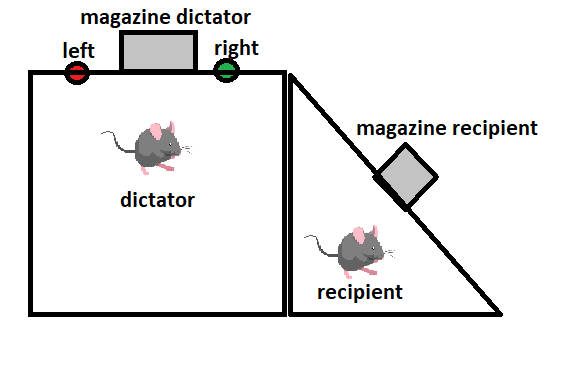
\includegraphics[scale=1.1]{altruism.png} 
	\end{center} 
	\caption{\textit{Main setting of the altruism task: a dictator mouse (left) can choose between two pokes, one of which will deliver a food pellet to a recipient mouse (right)}}
	
\end{figure}

The \textit{altruism task} is a task in which two mice are tested in their social decision making. It consists in two mice located in adjacent compartments, separated by a metal mesh which allows them to see and sniff each other, but not enter in direct contact. One mouse, called the \textit{recipient}, assumes only a passive role: it stays in its space and, when a food delivery happens from an apposite box (called \textit{magazine}) it can eat the delivered food pellet. 
In contrast, the other mouse, called \textit{dictator}, has to perform a social choice. Indeed, in any case a food delivery to its own magazine will happen by poking one of two buttons available, but even if both types of pokes will provoke a pellet delivery for the dictator, only one of them will give food to the recipient as well. It follows that the two choices of the dictator can be classified as \textit{selfish} and \textit{altruistic} decisions.\\
In order to stimulate the seeking for food, mice have been kept at $ 90 \%$ of their standard body weight before the test. The setup is organized as follows:

\begin{itemize}
	
	\item Before the tasks were performed, both mice were kept together in same sex pairs for two weeks 
	
	\item The animals were tested for $5$ days. The first day involves a \textit{learning} process for the dictator to understand the food delivery mechanism. The main test is considered to be during the following $3$ days, and finally the process is considered well assimilated by the dictator during the final day	
	
	\item The position of the altruistic and selfish pokes (i.e. of the two buttons providing or not the food delivery to the recipient) has been randomized through the different days of the test, in order to rule out spatial causes for the results
	
	\item A control test has been performed in parallel. Here, the recipient mice were replaced by inanimate objects, in order to determine the effective relevance of their presence in the task
	
	\item During the performance of the $5$ days of the test, the calcium activity in the basolateral amygdala of the dictator has been recorded using the Fiberphotometry technique, giving as result a collective signal (as discussed in Section 1.4)
	
\end{itemize}



\subsection{Behavioural results in the altruism task}


\begin{figure}[H]
	\begin{minipage}{\linewidth}
		\centering
		\begin{minipage}{0.46\linewidth}
			\begin{figure}[H]
				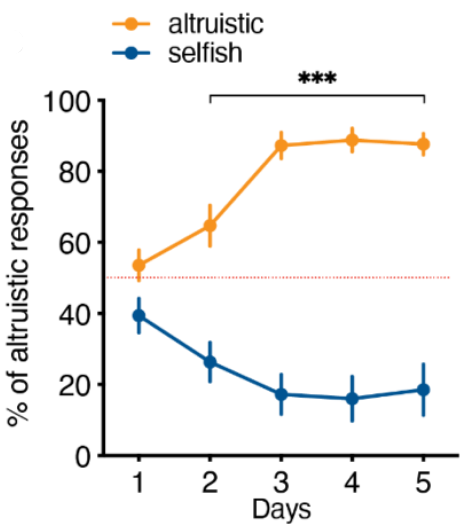
\includegraphics[width=\linewidth]{altr_self.png}
				
			\end{figure}
		\end{minipage}
		\hspace{0.05\linewidth}
		\begin{minipage}{0.46\linewidth}
			\begin{figure}[H]
				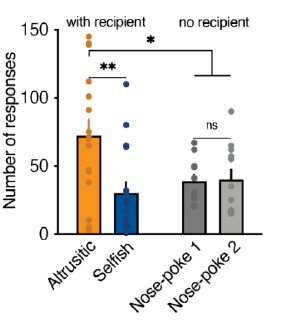
\includegraphics[width=\linewidth]{norecip.png}
				
			\end{figure}
		\end{minipage}
		
	\end{minipage}
	\caption{\textit{Left: Percentage of change in altruistic response (i.e in the number of altruistic pokes) for altruistic and selfish mice. Right: difference in number of altruistic and selfish pokes by the dictator when the recipient is present or not}}
\end{figure}



The first evident result of the altruism task is that, when a recipient mouse was present and same sex pairs adopted, the dictator mice showed an increase in the number of altruistic pokes during the test days. In contrast, when recipient mice were replaced by inanimate objects, no appreciable difference between altruistic and selfish preferences have been detected. Such differences started to emerge from the second day of the test, as confirmation of a successful learning period on the first day. \\
An important difference has been observed between male and female mice:  only male dictators showed altruism preference, while female ones did not show an appreciable difference between selfish and altruistic pokes.\\
Next, the spatial exploration of the mice has been performed. Results indicate that altruistic dictators (i.e.dictators which showed preference for altruistic pokes) tend to explore more the area in proximity to the recipient, in contrast with selfish dictators which did not show particular interest in their partners.\\
To test whether visual interaction plays a role determining the altruistic preferences, the task has been repeated replacing the metal mesh with an opaque screen, which still allowed olfactory and auditory stimuli, but not visual ones. In this situation, mice showed a marked decrease in the altruistic responses, with respect to the previous case in which a metal mesh was used. This implies that the dictator mouse needs to be able to see the recipient partner getting the food delivery, in order to be able to select the altruistic alternative.\\
Finally, to further determine the ability of the dictator mice to \textit{learn} from experience and change their habits in light of an altruistic choice, dictators were tested with no partner in adjacent cages, to trigger one nose poke over the other. Subsequently, the recipient mouse was put in the near cage, and the location of the altruistic poke, delivering food to it as well, has been assigned to the poke less pressed by the dictator. Despite this, the dictator showed through days a change in its preference towards the altruistic poke. Changing the recipient with an inanimate object, such preference decreased once again. The conclusion is straightforward: the presence of the recipient is the determining factor for the altruistic preference by the dictator.
\\

Once, in normal conditions, the altruistic preference has been established, one may ask under which conditions such preference is maintained. To this purpose, the task was repeated changing the rules of food delivering. Now, two nose pokes were necessary for the food delivery in the altruistic poke, while only one in the selfish one. Even with this additional effort, male and female mice which previously showed altruistic preferences, increased the number of altruistic over selfish preferences also in this case. Increasing the necessary number of pokes to $4$, male dictators kept their altruistic preferences, while female dictators did not show anymore a significant difference. Finally, requiring $6$ nose-pokes for altruistic delivery still kept male mice in their altruistic preference, while made female ones prefer the selfish one, and only from $8$ pokes, also males stopped to be altruistic. Overall, these results showed that \textit{male mice tend to share food with their cagemates partners, even at costly conditions}.\\
Finally, mice were tested in two more conditions: absence of rewards for both dictator and absence of reward for dictator, but not for the recipient mouse. While, in the first case, no preference between the two pokes was expressed by the dictator, in the second case there was an altruistic preference. This means that the dictator can choose an altruistic decision even if there is no direct benefit for itself.


\begin{figure}[H]
	\begin{center}
		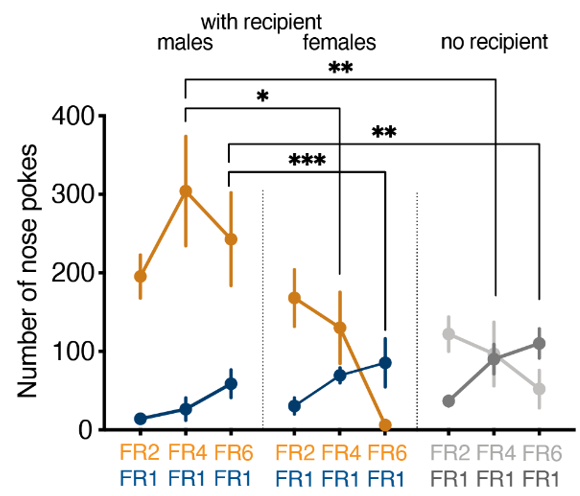
\includegraphics[scale=0.6]{number_pokes.png} 
	\end{center} 
	\caption{\textit{Number of nose pokes of male and female mice, with and without recipients.}}
	
\end{figure}

\subsection{The role of social hierarchy in altruism display}

\begin{figure}[H]
	\begin{center}
		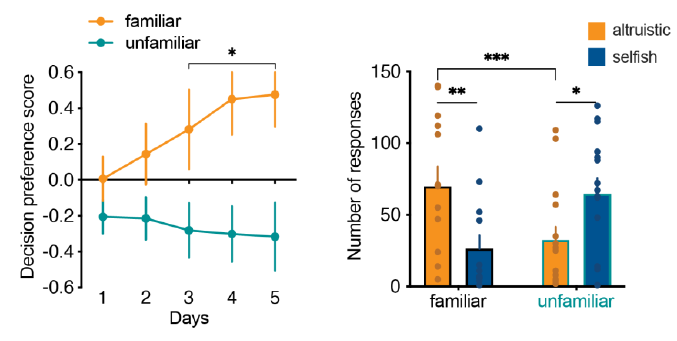
\includegraphics[scale=0.6]{familiar.png} 
	\end{center} 
	\caption{\textit{Left: decision preference score with familiar and unfamiliar recipients. Right: Number of responses by selfish and altruistic dictators, with familiar and unfamiliar recipients}}
	
\end{figure}

As of today, it has been recognized that familiarity between individuals plays a key role in social relationships [De Waal, F. B. M. \& Preston]. In the case of the altruism task, it is to be expected that the altruism shown by the dictator is strictly depending on the period preceding the test, in which dictator and recipient have been cagemates for two weeks. To test this hypothesis, the task has been repeated using unfamiliar recipients, showing no preference for altruistic choices, where indeed most of dictator mice showed preference for the seflish pokes. This has been measured through the \textbf{decision preference score} 

\begin{equation}
DPS = \frac{A -S}{A+S}
\end{equation}

where $A$ and $S$ are the number of altruistic and selfish responses, respectively.\\
Next, a \textit{dominant/follower} relationship has been established through the \textbf{tube test}, in which two mice have been paired in a tube allowing the passage of just one individual. This test helped to figure out whice of the two was the \textit{dominant} individual, i.e. the one pushing the other, and the \textit{follower} individual, i.e. the one retreating. The dominance was quantified through the \textbf{Normalized David's score} [De Vries, H., Stevens, J. M. G. \& Vervaecke]

\begin{equation}
NDS = \frac{1}{N}\left(DS + \frac{N(N-1)}{2}\right)
\end{equation}

where $N$ is the number of tested subjects and $DS$ is the David's score, i.e. the ratio of wins.\\
The analysis of 9 pairs of mice ($N=18$) yielded the main following results:

\begin{enumerate}
	\item The dominance relationship is \textit{transitive}: if mouse A is dominant with respect to mouse B, and mouse B is dominant with respect to mouse C, then mouse A dominates also mouse C 
	
	\item Dictator mice showing selfish preferences in the altruism task displayed low scores in the $NDS$ compared to their recipients, which means that selfish dictators  tend to be less dominant than their corresponding recipients
	
	\item No significant differences have been detected between the dominance scores of altruistic dictators and their recipients
	
	\item The more a dictator has a higher dominance value $NDS$, the more it is willing to perform altruistic preferences in the altruism task
	
\end{enumerate}

Next, the study tested the hypothesis that \textit{an increase in altruism is related to an increase in affective state matching between individuals}. To do so, the recipient has been subject to a manipulation of its emotional state, in this case a fear conditioning paradigm through mild shocks. In the meantime, the dictator mouse (here assuming the role of \textit{observer}) was allowed to see the recipient through a transparent separating wall.\\
The main result was that altruistic mice displayed an increased freezing behaviour during this phase, compared to selfish ones. Since these latter are the dominant ones, this result lead to the conclusion that \textit{dominant mice tend to show more empathic-like behaviours}, from altruism to emotional contagion.

\subsection{The role of BLA neurons in selfish and prosocial choices}

\begin{figure}[H]
	\begin{center}
		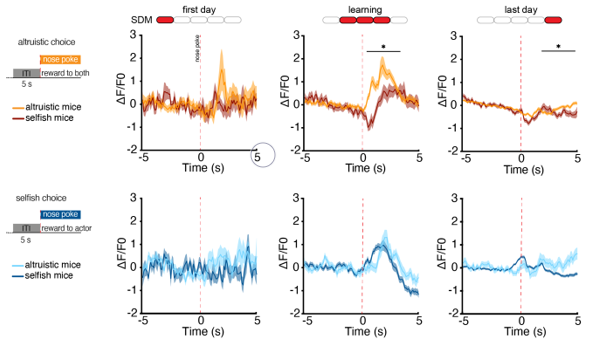
\includegraphics[scale=0.77]{psth.png} 
	\end{center} 
	\caption{\textit{Top row: PSTH of selfish and altruistic mice during nose pokes in altruistic pokes. Bottom row:  PSTH of selfish and altruistic mice during nose pokes in selfish pokes. Results have been averaged on all nose pokes}}
	
\end{figure}

The fiberphotometry analysis of the calcium activity in the BLA allowed to establish a connection between the type of choice adopted by dictator mice and their corresponding neural activity. In order to analyze the relative change of such activities during altruistic or selfish pokes, the raw data from the photometry have been subject to a \textbf{peristimulus time histogram (PSTH)} analysis. Such analysis goes through the following steps:

\begin{enumerate}
	
	\item Set a START and STOP time for the analysis, i.e. set the time window in which considering the variation of the neural activity (in this case START = STOP = $5 s$ for a window of $10 s$)
	
	\item For every time point $x_t$ of the overall activity given by Fiberphotometry, consider the interval $[x_{t}-START , x_{t}+STOP]$
	
	\item Compute the mean $ \mu_t$ and standard deviation $\sigma_t$ of the activity in such interval
	
	\item The value of the PSTH for the selected time point is then
	$$ P_t = \frac{x_t - \mu_t}{\sigma_t}$$
\end{enumerate}
Next, in order to quantify the intensity of the activity, \textbf{areas under the curve (AUC)} were estimated numerically using the trapezoid quadrature rule [Quarteroni-Sacco].\\

The overall analysis on raw photometry data, PSTH tracks and AUC showed some remarkable results:

\begin{itemize}
	
	\item Dictator mice showed an increased activity in the BLA when a recipient mouse was present, compared to the case where an inanimate object was placed in the near cage
	
	\item During the first and last day, in all cases no significant differences emerged in the activation of BLA
	
	\item In the intermediate days of learning, however, altruistic mice showed a strong activation during the nose poking in the altruistic pokes, but not in the selfish ones. Selfish mice, in contrast, did not show any particular activation of their neural activity during both pokes. 
	
	\item The AUC analysis suggested that the levels of activity were higher during the learning phase, rather than in the first and last day
\end{itemize}


To further inspect the role of BLA neurons in empathy display, such neurons have been silenced via a \textbf{chemogenetic procedure} [Qi-Gang Zhou, Ashley D Nemes]. In this approach, a viral vector, carrying specific receptors, is injected into the area of interest. Such receptors, called  \textbf{hM4D receptors}, belong to the group of \textit{inhibitory designer receptors exclusively activated by designer drugs (DREADD)}, which activate themselves only when in contact with a particular drug, the \textbf{Clozapine N-oxide (CNO)}. In this way, mice injected with hM4D-CNO will exhibit an \textit{inhibition} of BLA-neurons. In contrast a control group of mice was injected with CNO only, without hM4D receptors.\\
The obtained results after these injections showed a significant reduction of freezing behaviour in the dictators, while their recipient partners were subject to emotion conditioning as previously described. This confirms the conclusions of previous studies [Allsop, S. A. et al], namely a \textit{critical role of the amygdala in emotional matching}. Silencing BLA neurons revealed to be correlated also to the amount of altruism preferences. Indeed, mice with silenced BLA neurons failed to show a marked preference for altruistic choices, in contrast with the control case. Indeed, while approximately $3$ out of $4$ mice showed altruistic preferences in control conditions, a similar percentage of BLA-silenced mice showed preference for selfish pokes.\\
BLA silencing did not affect the number of responses or the latency of choices, rather it affected the type of the social decision. This is a further evidence of the primary role of BLA in altruism display.
\\
Finally,  silencing of BLA neurons appeared to reduce also the dominance: a higher number of BLA-silenced mice assumed a subordinate role with respect to control mice. In particular, if transitive relationships of dominance are distributed in levels $ \alpha \rightarrow \beta \rightarrow \gamma \rightarrow \delta $, silenced mice belong only to levels $ \gamma $ and $ \delta $.

\begin{figure}[H]
	\begin{center}
		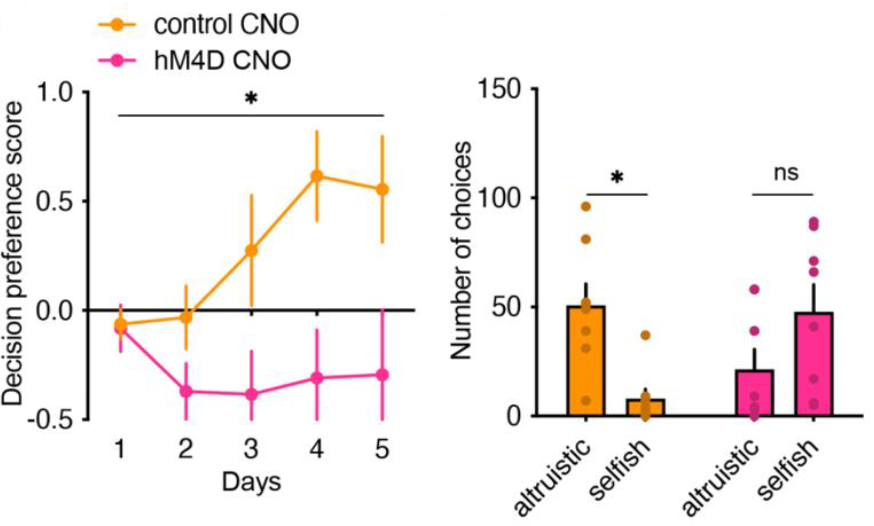
\includegraphics[scale=0.77]{silencing.png} 
	\end{center} 
	\caption{\textit{Left: Decision preference score in BLA-silenced mice (hM4D CNO) and non-silenced mice (control CNO). Right: number of selfish and altruistic pokes in BLA-silenced mice (hM4D CNO) and non-silenced mice (control CNO) }}
	
\end{figure}


\begin{figure}[H]
	\begin{center}
		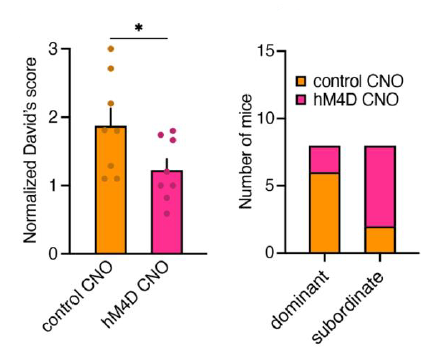
\includegraphics[scale=0.77]{sil_dom.png} 
	\end{center} 
	\caption{\textit{Left: Normalized David's score in BLA-silenced mice (hM4D CNO) and non-silenced mice (control CNO). Right: number of dominant and subordinate mice in BLA-silenced mice (hM4D CNO) and non-silenced mice (control CNO) }}
	
\end{figure}


\end{document}
